\appendix

\chapter{Notes}

\section{Mixins help reduce sharing constraints}
\label{sec:mixins-reduce-sharing-constraints}

The goal of this appendix is to explain why mixins help ``avoid the
preponderance of sharing constraints that occur with ML functors.''
(as claimed in Section~\ref{sec:intro})  For concreteness, the ML
examples in this section will be written in OCaml.

\paragraph{What is a sharing constraint?}
Ordinarily, an abstract type in a signature is not equal to any other type.  A
sharing constraint \verb|with type t = u| asks the compiler to expose
the fact that the abstract type \verb|t| is equal to some other type \verb|u|.%
\footnote{For the language lawyers out there, SML also defined a
construct \texttt{sharing type} which is a specialized signature
refinement operator for specifying that two abstract type components
inside a signature are transparently equal (the \texttt{with type} construct
doesn't suffice for this case, since an abstract type defined inside
the signature is not a valid type outside the signature.) We'll use
the colloquial meaning of sharing constraints to refer to both constructs.}
In ML, sharing constraints are needed most commonly in two situations:

\begin{enumerate}
    \item When a module is \emph{sealed} by some signature, a sharing
    constraint may be used to reveal some types which would otherwise
    be opaque. For example, consider these modules for maps with arbitrary
    keys:

\begin{lstlisting}[language=ML]
        module IntMap =
          struct
            type key = int
            type 'a t = ...
            let insert k v m = ...
          end
        module type MAP =
          sig
            type key
            type 'a t
            val insert : key -> 'a -> 'a t -> 'a t
          end
        module SealedIntMap = (IntMap : MAP)
\end{lstlisting}

    \noindent In this example, the resulting \verb|SealedIntMap| has
    an opaque \verb|key| and \verb|t| type, because it was sealed
    with the signature for \verb|MAP|.  However, there is a problem
    with \verb|SealedIntMap|: we don't
    know anything about the type of \verb|key|, and thus cannot actually
    use \verb|insert| (because we can't produce a value of type \verb|key|).

    A sharing constraint allows us to add a constraint to the signature \verb|MAP|
    saying, ``And actually, \verb|key| is an \verb|int|'':

\begin{lstlisting}
    module BetterSealedIntMap = (IntMap : MAP with type key = int)
\end{lstlisting}

    \noindent We won't say much about this use case, because \Backpack{} does
    not support sealing, so there isn't a point of comparison.

    \item A sharing constraint may be used to relate types between multiple
    signatures, which specify arguments to a functor.  For example:

\begin{lstlisting}[language=ML,escapechar=@]
    module type A = sig type t;; val f : t -> t end
    module type B = sig type t;; val g : t      end
    module F (X : A) (Y : B with type t = X.t) = struct let z = @\fbox{X.f Y.g}@ end
\end{lstlisting}

    Here, \verb|X.t| and \verb|Y.t| are not type equal without the
    sharing constraint \verb|with type t = X.T| on \verb|B|; without
    the sharing constraint, the boxed \verb|X.f Y.g| would not typecheck.

\end{enumerate}

\noindent
In fact, \Backpack{} also supports sharing constraints: for example,
if an inherited signature defines an abstract type \verb|data T|, we
can define a local signature at this name with the declaration \verb|type T = Int|
to refine the abstract type \verb|T| into \verb|Int|.

\paragraph{How does Backpack eliminate sharing constraints?}  In a mixin
module system like \Backpack{}, a sharing constraint is implicitly generated
whenever two types are brought into scope under the same name.  For example,
if I depend on two packages which both require an implementation of
\verb|Str|, the two signatures will be merged together, so that \verb|Str|
from the signature of the first package and \verb|Str| from the signature
of the second package are treated as the same type.

An analogous situation in ML occurs when I have two functors,
which I would like to instantiate with the same module:

\begin{lstlisting}[language=ML,escapechar=@]
    module type A1 = sig type t;; val f : t -> t end
    module type A2 = sig type t;; val g : t      end
    module F1 (X : A1) = struct ... end
    module F2 (X : A2) = struct ... end
    module F (X : @\fbox{???}@) = struct
        module M1 = F1(X)
        module M2 = F2(X)
        ...
    end
\end{lstlisting}

\noindent
What signature can we can we give here?  Unlike in \Backpack{}, we must
specify the signature.  One possibility is to write the merged signature
by hand:

\begin{lstlisting}[language=ML,escapechar=@]
    module type A =
      sig type t
          val f : t -> t
          val g : t
      end
\end{lstlisting}

\noindent
This may be tiresome if the signatures are large.  Fortunately,
ML also supports the \verb|include| construct, which textually includes
the contents of a signature into a new signature, which can be used to
construct the merged signature by including both signatures.  However, there is a twist:

\begin{lstlisting}[language=ML,escapechar=@]
    module type A =
      sig include A1
          include A2 with t := t
      end
\end{lstlisting}

\noindent
We must relate the \verb|t| from \verb|A1| with the type \verb|t| from
\verb|A2|. In OCaml, we can
declare this relationship with a \emph{destructive substitution}.
The destructive substitution \verb|type t := t| says, ``Find all occurrences
of \verb|t| inside \verb|A2|, replace them with the \verb|t| that is in
scope (from \verb|A1|), and delete \verb|type t| from \verb|A2|.''
The final signature is equivalent to the one we wrote out by hand.

Destructive substitution only works for types, so if two signatures
define the same functions or values, your only recourse is to write the
merged signature by hand, or pass in two modules, one for each signature,
with the necessary sharing constraints to witness the necessary type equalities
(as seen in the example functor with two module arguments).

\paragraph{Summary}
\Backpack{} doesn't eliminate all cases where sharing constraints might be
useful; for example, a user of \Backpack{} may still find it useful to
declare \verb|type Key = Int| to refine the type of an abstract map
to be a map with integer keys.  However, it does eliminate one important
class of sharing constraints which arise when there are multiple signatures
describing the same types and functions.

%   \begin{tabular}{p{0.45\textwidth} p{0.45\textwidth}}
%   \begin{lstlisting}[language=ML]
%   module type A1 = sig
%       type t = int
%       type u
%       val f : int -> u
%   end
%   \end{lstlisting}
%   &
%   \begin{lstlisting}[language=ML]
%   module type A2 = sig
%       type t
%       type u = bool
%       val f : t -> bool
%   end
%   \end{lstlisting}
%   \end{tabular}


%   Sharing constraints in ML permit users to specify that two modules
%   specify the same abstract type.
%   Here is an example application of
%   sharing constraints in OCaml adapted from the OCaml FAQ\footnote{\url{https://caml.inria.fr/resources/doc/faq/module.en.html}}:
%   \begin{lstlisting}[language=ML,escapechar=@]
%       module type S1 = sig type t
%                            val x : t
%                        end
%       module type S2 = sig type t
%                            val f : t -> t
%                        end
%       module F (X : S1) (Y : S2 with type t = X.t) =
%         struct
%           let g = Y.f X.x
%         end
%   \end{lstlisting}
%   %
%   In this example, the signatures \verb|S1| and \verb|S2| both define
%   an abstract type \verb|t| and some values which operate on this type.
%   When we define a functor \verb|F| which takes a module of type \verb|S1|
%   and a module of type \verb|S2|, it is \emph{not} automatically the case
%   that the \verb|t| from \verb|X| and the \verb|t| from \verb|Y| are the same.
%   To declare that these types are the same, we specify a sharing constraint
%   \verb|with type t = X.t| which declares the equality between \verb|X.t|
%   and \verb|Y.t|.

\chapter{Recursive linking}
\label{sec:recursive-linking}

In this section, we sketch how to add support for recursive linking to
\Backpack{}, allowing us to mix-in link libraries which recursively
depend on each other.  Even though \Backpack{} as described in this
thesis does not support recursive linking, many aspects of its design
(e.g., mix-ins) were inherited from systems which did support recursive
linking (notably, \OldBackpack{} and MixML).

%   We will first informally describe how to make use of recursive
%   linking in \Backpack{}, pointing out some subtleties that arise
%   in the presence of recursive linking.  Then we will sketch semantics
%   for recursive linking, and 

\section{A simple example}

Suppose that you have modules implementing logging and database access,
with the following interfaces:

\begin{lstlisting}
    signature Logging where
        data LogHandle
        log :: LogHandle -> String -> IO ()

    signature Database where
        data DbHandle
        data Query a
        query :: DbHandle -> Query a -> IO a
\end{lstlisting}
%
A cyclic dependency may arise if the database service logs queries with
the logging API, but you have a database-backed logger which is
implemented using the database API\@.\footnote{Let us not consider the
wisdom of logging to a database or structuring the API this way.}  In
conventional Haskell, we can place these in separate modules and break
the cyclic imports with an \verb|hs-boot| file:

\begin{lstlisting}
    -- Database.hs-boot
    module Database where
        data DbHandle
        data Query a
        query :: DbHandle -> Query a -> IO a

    -- Logging.hs
    module Logging where
        import {-# SOURCE #-} Database
        data LogHandle = ...
        log :: LogHandle -> String -> IO ()
        log = ...

    -- Database.hs
    module Database where
        import Logging
        data DbHandle = ...
        data Query a = ...
        query :: DbHandle -> Query a -> IO a
        query = ...
\end{lstlisting}
%
If you want to place \verb|Database| and \verb|Logging| in separate
packages, \verb|hs-boot| files are insufficient---\Backpack{} with
recursive linking, however, will get the job done:

\begin{lstlisting}[language=Cabal]
    -- database.cabal
    name: database
    library
      exposed-modules: Database
      signatures: Logging

    -- logging.cabal
    name: logging
    library
      exposed-modules: Logging
      signatures: Database
\end{lstlisting}
%
If a package depends on both \verb|database| and \verb|logging|,
\verb|database|'s \verb|Logging| requirement will be filled with \verb|logging|,
and vice versa.  Alternately, \verb|database| can have a direct
dependency on \verb|logging|, filling \verb|logging|'s requirement with a module
it defines locally.

\begin{lstlisting}[language=Cabal]
    -- logging.cabal as before

    -- database.cabal
    name: database
    library
      build-depends: logging
      exposed-modules: Database
\end{lstlisting}

\paragraph{Comparison with \OldBackpack{}}
In \OldBackpack{}, signatures subsume \verb|hs-boot| files, because a signature
and a module can be defined in the same package:

\begin{lstlisting}
    package p where
        Database :: [ ... ]
        Logging  = [ import Database; ... ]
        Database = [ import Logging; ... ]
\end{lstlisting}
%
Although we briefly attempted to implement this design, we eventually
decided to keep \verb|hs-boot| and \verb|hsig| files as distinct
concepts.  The big problem is that \OldBackpack{} assumes an explicit
user-specified ordering on the modules and signatures in a package,
while Haskell code written in the wild today assumes an implicit
ordering specified by the import statements in modules.  There is no
convenient way to specify how a module and its signature should be
ordered relative to other modules, without adopting an \verb|hs-boot|
style \verb|{-# SOURCE #-}| import syntax.

\section{Challenges}

The presence of recursive linking introduces new complications for
type checking.

\paragraph{Cyclic exports}  Consider the following recursive module
definition:

\begin{lstlisting}
    -- package b
    signature A where
        x :: Int
    module B(x) where
        import A(x)
    -- package a, which depends on b
    module A(x) where
        import B(x)
\end{lstlisting}

In Haskell, an implementation cycle isn't necessarily a problem,
because a binding like \verb|x = x| can simply be compiled into a thunk
which infinite loops when forced.  However, what should be the original
name of this \verb|x|?  There is no appropriate name, because there
isn't any module (not signature) which ever defines \verb|x|.  Thus,
recursive \Backpack{} must reject this implementation.

(\verb|hs-boot| files do not suffer from this problem, because GHC
Haskell does not permit entities in an \verb|hs-boot| file to be implemented
using a reexport.)

\paragraph{No backwards propagation}
GHC is an incremental compiler: if you edit a module of a previously
compiled project, only modules which transitively import it need to be
recompiled.  For this strategy to be correct, it must not be the case
that a downstream module can affect the compilation of an upstream one.
Unfortunately, the \emph{shaping pass} of \OldBackpack{}---used to
prevent the double vision problem---is a pre-pass
which can cause information to propagate backwards.  Consider the
following example:

\begin{lstlisting}[escapechar=@]
    package p where
        A :: [ data T ]
        B = [ import A; f (x :: T) = x ]
    package q where
        include p
        I = [ data T = MkT ]
        C = [ import B; import I; y = @\fbox{f MkT}@ ]
        A = [ exports (T); import C; import I(T) ]
\end{lstlisting}
%
Here, the shaping pass determines that the abstract \verb|T| from
\verb|A| and the concrete \verb|T| from \verb|I| coincide, ensuring that
the enboxed \verb|f MkT| will typecheck.  We can see that if we
modify the implementation of \verb|A| (last line) to define a different
\verb|T|, this equality would no longer hold, and \verb|C| would
fail to typecheck.  Thus, information propagates backwards from
the implementation of \verb|A| to \verb|C|.

In \Backpack{}, we propose that \verb|f MkT| should \emph{not}
typecheck, in order to preserve incremental compilation.  More
generally, only the implementor of a module and any modules which
transitively import it should be affected by any refinements to original
names that occur due to exports in the implementation of a module.
Consequently, we refine the original names of a forward reference only
immediately before we typecheck the implementation of this forward
reference.

%   Lack of backwards propagation also causes a technical difficulty in
%   implementation: after type checking modules, we may need to write out
%   references to as yet to be resolved hole variables (which will later be
%   recursively defined), on faith that they will be backpatched to the
%   correctly values later.

%   This change also allows us to sidestep some infelicities with
%   \OldBackpack{}'s shaping pass:

%   \begin{lstlisting}[escapechar=@]
%       package p where
%           A :: [ data T ]
%           B = [ exports (T); import A ]
%       package q where
%           include p
%           I = [ data T = MkT ]
%           C = [ @\fbox{exports (T)}@; import B; import I ]
%           A = [ exports (T); import I(T) ]
%   \end{lstlisting}

%   Under \OldBackpack{}'s backwards propagating semantics,
%   we might say that \verb|C|'s export of \verb|T|
%   is unambiguous (because of the implementation of \verb|A|).
%   However, \OldBackpack{} will reject \verb|C| during
%   shaping, because at the time of shaping, we must resolve the export of
%   \verb|T|, but it is not known that \verb|I.T| and \verb|B.T| coincide
%   (that's what shaping is trying to figure out!)  In principle, this
%   problem could be solved by a more sophisticated shaping algorithm,
%   but this is 

\paragraph{Translucency}  A feature not supported in \OldBackpack{}
but supported in \Backpack{} is
the ability to use a type synonym to implement an abstract data type.
This introduces a form of ``translucency'', where the abstract data type
is opaque while the implementation is unknown, and transparent afterwards.
For example, in Section~\ref{sec:instantiating-the-matcher}, we demonstrated
how we could instantiate a generic regular expression matcher to match on strings.
Inside the implementation of the matcher, we knew nothing about the abstract
type \verb|Str|; after instantiating it, the \verb|accept| function
transparently accepts \verb|String| arguments.

Translucency introduces yet another variant of the \emph{double vision}
problem.  In systems like RMC and MixML, double vision is solved by
introducing a type precomputation pass, which means that we end up
with same kind of backwards propagation we described in \OldBackpack{}.
Here is the analogous example, rewritten to use translucency rather than
exports:

\begin{lstlisting}[escapechar=@]
    -- package p
    signature A where
        data T
    module B where
        import A
        f (x :: T) = x
    -- package q, which depends on p
    module C where
        import B
        y = @\fbox{f 2}@
    module A where
        import C
        type T = Int
\end{lstlisting}
%
Here, we provide a forward declaration of \verb|A| which
declares \verb|T| abstractly, which is eventually declared to be
a type synonym of \verb|Int|.  The key expression is boxed: does \verb|f 2|
in module \verb|C| typecheck?

Just as we argued previously, we think \verb|f 2| should \emph{not}
typecheck.  If we were to move the definition of \verb|y| to \verb|A|
(or any module that imports \verb|A|) it should typecheck in all cases.
This is in contrast to the behavior of MixML\@:

\begin{figure}[H]
\begin{tabular}{p{0.40\textwidth} p{0.50\textwidth}}
\begin{lstlisting}[language=ML,escapechar=@]
link X = { type t }
with ( { val f (x : X.t) = x,
         val y = @\fbox{f 2}@ }
           with
       { type t = int } )
\end{lstlisting}
&
\begin{verbatim}
(* mixml 0.2.1 passes with type: *)
it : {f : [int -> int]+,
      t : [= int : #],
      y : [int]+}
\end{verbatim}
\end{tabular}
\caption{Backwards propagating type information in MixML}
\label{fig:double-vision-backwards-propagating-mixml}
\end{figure}

\noindent
Although we have very loosely translated the example (a more
faithful example would actually construct \verb|f|, \verb|y| and
\verb|t| in substructures representing each Haskell level
module), the same basic pattern holds: when typechecking \verb|f 2|,
\verb|X.t| is already known to be equal to \verb|int|.

\section{Recursive \uid{}s}
\label{sec:recursive-uids}

%   **Warning:** The extension described in this section is not implemented
%   in GHC 8.2.  It can be skipped upon a first reading.

\Backpack{} with recursive linking requires generalizing unit
identifiers to be infinite regular trees.  As was the case
in \OldBackpack{}, these trees can be
represently finitely using $\mu$-binders (ala recursive types),
with the following abstract syntax (where $\alpha$ ranges over
unit identity variables):

\[
\begin{array}{rcll}
  \UP &::=& \mu\alpha.\, \icid{\Up}{S} & \text{\Uid} \\
      & | & \alpha \\
\end{array}
\]

%   A more parsimonious extension to the concrete syntax is to
%   have every ``ComponentId`` "constructor" implicitly introduce
%   a μ-binding, and represent the variables with de Bruijn indexes.
%   Let ``UnitIdVar`` range over natural numbers, then:

%   ::

%       UnitId ::= ComponentId "[" ModuleSubst "]"
%                | UnitIdVar

Pictorially, recursive components simply relax the acyclicity restriction on
the component graph:

\begin{figure}[H]
\center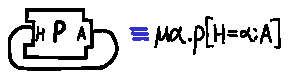
\includegraphics{figures/recursive-unit-identifier.pdf}
\end{figure}

These graphs are equivalent up to unfoldings (i.e., unrolling the
cycles).
As observed in \OldBackpack{}, infinite trees of this form
can be tested for equivalence using Huet's unification algorithm.
However, for an implementation, it is more convenient to compute the canonical form
of a \uid{}, so equality can be checked syntactically.  This can be
computed by Moore machine minimization.  Canonicalization can be achieved
in three steps:

\begin{enumerate}
\item Convert the unit identifier into a Moore machine,
\item Minimize the Moore machine (the procedure is similar to DFA
   minimization, except that states with differing outputs are
   initialized to be in separate equivalence classes initially), and
\item Convert the Moore machine back into a unit identifier.
\end{enumerate}
%
Intuitively, the Moore machine of a unit identifier recognizes paths
(from right to left) through the component graph, outputting the
component identifiers of the component boxes it traverses.

\begin{figure}[H]
\center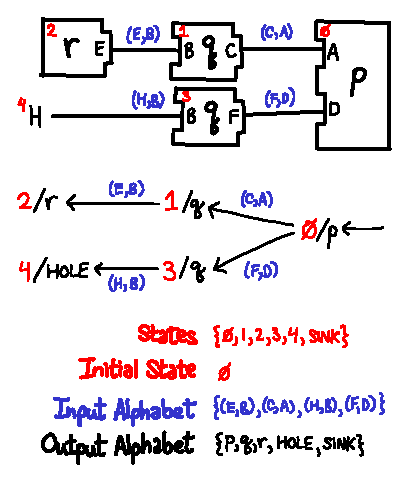
\includegraphics{figures/moore-description.pdf}
\end{figure}

\noindent
Formally, we define the partial Moore machine corresponding to a unit
identifier as follows:

\begin{enumerate}
\item The state set ranges over component boxes and hole modules in the
   graph (in the diagram above, we simply assigned a number to each
   box/hole).
\item The input alphabet is the Cartesian product of output module names
   and input module names.  Intuitively, each member of the alphabet
   corresponds to a wire labeled with the name of the input and output
   ports it is wired to.
\item The output alphabet is the set of component identifiers, as well
   as a distinguished element \verb|HOLE| for hole modules.
\item The inital state is the state corresponding to the component box of
   the unit identifier we want to denote.
\item A transition from $q$ to $q'$ on the input $(m, m')$ exists
   if there is a wire from the input port $m'$ of $q$ to the output
   port $m$ of $q'$ (or a hole module $\hv{m}$, if $q'$ corresponds to a hole
   module).
\item The output of a state is the component identifier of its component
   box, or \verb|HOLE| if it is a hole module.
\end{enumerate}
%
We can complete the partial Moore machine into a total Moore machine by
adding a new sink state \verb|SINK|, which outputs a new output value
\verb|SINK|, and directing all undefined transitions to it (not depicted on
the diagram).

Here are two examples of recursive components expressed as Moore
machines:

\begin{figure}[H]
\center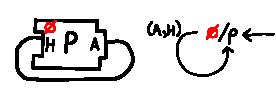
\includegraphics{figures/moore-p.pdf}
\hspace{3em}
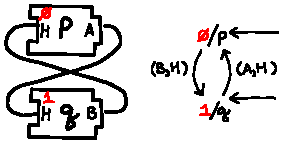
\includegraphics{figures/moore-pq.pdf}
\end{figure}

\noindent
The \uid{} corresponding to a Moore machine is defined by
recursively traversing the Moore machine, creating unit identifiers
whose component identifier is the output at a state, and module
substitution is all of the outgoing transitions to non-sink states. During
this traversal, we maintain a stack of seen states:  when we reach a
state that is already on our stack, we emit a variable bound
for that state on the stack.  This traversal
is guaranteed to terminate as the size of the state set is finite.

\section{Mix-in linking}

Mix-in linking can be straightforwardly adapted to a recursive
setting: the algorithm proceeds as before, but we remove the
occurs check from unification, allowing our unification to
produce infinite trees (as describe above.)  Pictorially,
this simply corresponds to allowing loops when we wire up provisions
to requirements in our component shapes.

\section{Type checking}

The primary complexity in handling recursive linking comes in adapting
typechecking in GHC to operate in this new regime and correctly
handle double vision.

For example, consider renaming.  Ordinarily, renaming of a module
proceeds by looking up the exports of each module, and then computing
the original names of reexports using the subsequent environment.
To lookup the export of a module, we first need to instantiate it.
The crux of the matter is that if the module occurs recursively
within the module identifier, then we need the exports of our module:
but we cannot provide them, because we are still in the process
of computing them.  A partial solution is to treat these abstractly,
and then refine them afterwards (shaping pass), but there is one
more detail, which is that we have to defer concluding that exports
are ambiguous due to the abstract types, because they may not be
ambiguous after refinement.  (Also, necessity to bottom out if an
instantiation cuases a loop.)

Now consider typechecking.  Here, the issue is a bit easier, because
there is already a built-in type computation pass in GHC already,
where we first handle all type declarations, before handling anything
else.  There is one technical obstacle, which is that we have to make
sure that the merged types of this module pass through this mechanism.
Blah blah blah.

So the crux of the matter is handling lookup.  Another problem is
when you hit a lookup for something that hasn't been locally handled
yet.  On the fly UN-CHECKED merge necessary.  (When things get refined to other
things.)

Dependency typing needs to stop testing once we reach
recursion. Intuitively, you only have to check the
LINKAGES for well-typedness, and there are finitely
many of them.



typecheck signatures in the local import order
    when they reach for types that are not locally defined, grab them
    from merged environment (merged on the fly ugh)

    problem: outer signature T imported S, but you have S import T.
    Your S refines a type so that T will typecheck. T is not allowed
    to see it. RIGHTLY SO.

SIGNATURES D: D: D: D:

Complication: handling hole variables that are going to be filled
by another module in the same package.

Typechecking-compilation works as a pre-pass to allow you to
get the export information.  (But wait! We assume that if you have
no holes we can skip typechecking. Ouch.)  Alternate strategy:
point these at specially munged forward decls, then add the
correct names afterward.  Precedent: dictionaries.

Difference between exports and type synonyms. Exports is harder
in some sense.



STOP STOP STOP

The basis for supporting recursive typechecking follows the same
machinery which allows Haskell to support recursive type definitions
inside of a module without any trouble: the basic principle is to

\section{Double vision}


OUTLINE

How can Backpack support recursive linking?
What do we mean by recursive linking?
    Standard set by MixML / Backpack'14
    Principle of ``no backwards flow''
How does GHC handle recursive definitions?
    Relationship with type computation pass
Laying down the semantics
    Renaming
    Typechecking
In what sense do we solve double vision?
    The easy sense
    NOT with sealing



\Backpack{}'s mix-in based design means that it is easy to express
build recursively linked components





Let's start by talking about recursive definitions within a single
module.  Within a single module, Haskell type and value declarations
are permitted to rely on each other arbitrarily, without forward
declarations.  How does the compiler untangle this mess?  It computes
a dependency graph of strongly connected components, and then kind-checks/type-checks
the components all at once.  Importantly, there never is a dependency
from a value to a type (modulo Dependent Haskell; but even then, if
you don't have induction-recursion you can't end up in a situation where
a value and a type have a recursive dependency.)  This means we can go ahead
and kind check all type declarations before doing any value-level type
checking.

This strategy for typechecking recursive declarations closely mirrors
proposals for handling recursive modules, i.e., in RMC and MixML\@; however,
instead of posing the problem as a ``staging'' (process types, the process
values), the problem is posed more as ``pre-pass'' (run the typing rules in
type computation mode, skipping values, and then run the full typing
rules with everything.)  This is one of those cases assuming your language
can do some sort of dependency analysis comes quite in handy (and prevents
you from making decisions in your design that would rely on ordering).

So, assuming you have a compiler that knows how to deal with recursive
definitions in one module, this gives you a basis for how any sort
of recursive linking should work, which is that you should be able to,
in principle, copy paste everything into a single module and typecheck it.
Obviously, you need name everything appropriately (identities, ding ding)
but this should give you an idea for what should work, and what shouldn't work.

When people say that double-vision is difficult, they are working in the
context of the ML module system, which has far more sophisticated \emph{sealing}
mechanism, which makes things more complicated.  Think about this:

\begin{verbatim}
seal T where
    type T = Int
    f :: T -> (U, T)
    f x = let (y, z) = g (x + 3)
          in (y, z + 3)

seal U where
    type U = Bool
    g :: T -> (U, T)
    g x = ... f ...
\end{verbatim}

How would you go about typechecking things?  The obvious strategy was to typecheck
each seal individually, and then generate the abstract types and apply coercions.
But now there's a recursion so you can't do that.  Another idea is to typecheck
the types first, and then handle the values.  But what are you going to put into
the context: the sealed version or the unsealed version? You need different things
in each case. Well, you can make it work and then it looks like MixML\@.

If you don't care about data abstraction, recursive linking is easy, because you
setup all the types first, and then you typecheck everything else.  There is one
further complication, which is that you may have forward declared things, you might
have a pile of stuff in the context which was typechecked relative to an abstract
type.  But that's not a problem either, because you can arrange to only ever look at
the KINDs of the forward declarations (which are perfectly well declared) until
you've setup your context.  This is literally how GHC does it.  I don't think the
algorithm is written down anywhere but that's how it is.


So, hypothetically, if we wanted to support recursive linking in Backpack,
here's how we'd do it.

First, we'd bring back recursive module identities, so that we can actually
give names to these things.

Now let's talk about how we instantiate in the presence of recursion.
Ordinarily, when we want to instantiate an interface, we look at the
module that instantiated it to figure out how to apply a name substitution.
Whatever we do, it has to bottom out; if we get to the point where we need
to lookup the same interface to determine the identity of the thing, that means
we are recursively reexporting ourselve (and not going to get anywhere), so
bail out.  Just cycle check.

The crux of the matter is whether or not a module from the package I'm currently
INDEFNITE typechecking, FURTHER DOWNSTREAM, can show up in dependency.
Yes it can, if we allow arbitrary mix-in linking.

\begin{verbatim}
package q where
    signature B where
        f :: Int
    module S(f) where
        import B
package p where
    include q
    module P where
        f :: Int
        f = 3
    module A(f) where
        import S
        import P
    -- CUT
    module B(f) where
        import A ()
        import P
        -- versus f :: Int; f = 2
\end{verbatim}

Essentially, we can construct situations where it is impossible to
know whether or not A should typecheck without having renamed B.
\OldBackpack{} said, ``OK, so clearly, we should run a shaping pre-pass
to solve this problem.''  But this is awful from a recompilation perspective;
we really don't want to be in the business of having to recompile when B
changes.  (By the way, how bad is recompilation with recursive linking
acros packages? Let's not talk about that for now\ldots)

So, the claim is \OldBackpack{}, with its shaping pass, is solving a
problem that people didn't really want solved in any case.  But the crux
of the matter is how to setup a reasonable restriction which will rule
out these shenanigans.  One answer is to disallow instantiating
dependencies with modules that you are defining in this package, but
this may require annoying gyrations moving modules out to separate
libraries and creating new signatures for their missing deps (it's
always possible, but not always pleasant).  Another compromise is
hs-boot assumptions about where a recursively defined entity is going to
be imported from.  Yet another compromise is to NOT make assumptions
about the true name of f (but that is irritating because you have to
backpatch in the hole instantiation on the interface when loading. But
it's doable.)

OK, so supposing you set this up correctly, when it comes to typechecking,
you have a similar problem which is whether or not you should ``see backwards''.
We argue you shouldn't, it should be opaque until you're actually at the
module.  Now there is something very lovely, which is that a type synonym
never actually gets replaced with the actual thing, so there's always a marker
we can look at which forwards us to the correct definition later (that's why
context improvement works.)

And finally, when we define a type within a module itself, does it get updated
throughout the context before we handle types within the same module? Sure
why not; because we have STAGING (this is how hs-boot knot-tying works.)

A key limitation of \Backpack{} as described in this thesis is its
lack of support for recursively linked modules.  Recursive modules
are generally thought to be difficult to typecheck due to the
\emph{double vision} problem, which occurs when the things an
implementing module knows about a type do not coincide with the
things they know about the recursive occurrence of that very same
type.


Compilers like GHC are able to handle recursive type and value
definitions within a single module without any trouble.


Prior literature suggests that a type computation \emph{pre-pass}
is necessary to get everything in order before performing type
checking proper.



It's just a simple matter of 


tl;dr The Haskell typechecker supports typechecking recursively
defined types and functions without trouble, in part because it
does not seek to support some of the features which recursive
modules in ML want to support (sealing).  Recursive modules in Haskell
should be understood in terms of this existing recursive support; indeed,
the existing \verb|hs-boot| mechanism (which \OldBackpack{} relies critically
upon in order to implement recursive linking) is achieved this way.


How does hs-boot work?  Like most ``simple'' formulations of the
recursive module rule, an hs-boot file initially operates by placing
some (to-be-defined) types and functions in the environment, which
modules can use.  Eventually, we typecheck the module which implements
the signature.




\Backpack{} as described in this thesis does not support recursive
linking. This is despite the fact that its predecessors, \OldBackpack{}
and MixML, held up the ability to handle recursive modules as one of
their chief technical achievements.  This raises the question: can
\Backpack{} be extended to support recursive linking?  Can the solutions
from \OldBackpack{} and MixML be directly applied with \Backpack{}?  If
not, what would the design of a recursive \Backpack{} be?


One decision we made when embarking on the design of \Backpack{}
was to \emph{not} handle the problem of recursive linking.  Initially,
\Backpack{} was not too different from \OldBackpack{} (which did
support recursive linking)

A big limitation of \Backpack{} is the fact that it does not support
recursive linking.  

The purpose of this section is to sketch a design for an extension to
\Backpack{} which supports recursive linking.  This is not a trivial
application of ideas from \OldBackpack{} (which did support recursive linking)
because \Backpack{} also introduces translucency (the ability to define
an abstract data type using a transparent type synonym), which \OldBackpack{}
did not support.  Nor is it a trivial application of ideas from MixML
(which did support translucency), as we seek to support type checking
in a \emph{single} pass over modules, as this property is essential
to usable recompilation avoidance in a real compiler.

Any semantics of recursive modules must grapple with the \emph{double
vision problem}.  First coined by Dreyer in his
thesis~\cite{dreyer:thesis}, the double vision problem refers to
technical difficulty that arises when attempting to define the typing
rules for recursive modules.  Informally, the double vision problem
occurs when the things an implementing module knows about a type does
not coincide with the things they know about the recursive occurrence of
that very same type.

There is no formal definition of ``double vision'', which at times makes
it difficult to characterize, because module systems can solve double
vision to varying degrees---arguably, even \Backpack{}, which has no
recursive linking, solves a variant of the double vision problem when
performing signature merging.  We will see that MixML and \OldBackpack{}
solve \emph{stronger} versions of the double vision problem, necessitating
a type/shape-computation prepass.  If one weakens the problem, the
need for a prepass vanishes.

This section is structured as follows.  First, we will characterize the
double-vision problem by giving a number of litmus tests which
demonstrate the problem in existing module systems; then, we'll describe
precisely in what sense can the double-vision problem be solved in
\Backpack{} without a prepass.

\section{Simple recursion}

\paragraph{Simple recursion in OCaml}  Our first litmus test is a simple
recursive module from Rossberg\footnote{\url{http://caml.inria.fr/pub/ml-archives/caml-list/2007/05/d9414d45a9a6f30f2609e08c43f011a0.en.html}}, which fails to compile in OCaml 4.02:

% chktex-file 13
% chktex-file 26
% chktex-file 36
\begin{figure}[H]
\begin{tabular}{p{0.35\textwidth} p{0.55\textwidth}}
\begin{lstlisting}[language=ML,escapechar=@]
module rec A : sig
  type t
  val f : t -> t
end =
struct
  type t = int
  let f (x : t) = A.f @\fbox{x}@
end
\end{lstlisting}
&
\begin{verbatim}
(* OCaml 4.02.03 fails with: *)
Error: This expression has type t = int
       but an expression was expected of type A.t
\end{verbatim}
\end{tabular}
\caption{Simple recursion in OCaml with type synonyms}
\label{fig:double-vision-simple-recursion-ocaml-synonym}
\end{figure}

\noindent
OCaml has determined the type of \verb|A.f| to be \verb|A.t -> A.t|,
while the boxed \verb|x| has type \verb|t|.  This example exhibits
``double vision'' because OCaml is unable to tell that \verb|A.t| and
\verb|t| are equal, despite the fact that, ``intuitively'', both identifiers refer to
the same type.

A slight variation on the above litmus test is one which utilizes a generative type
definition (\verb|type t = MkT of int|) rather than a type synonym (\verb|type t = int|):

\begin{figure}[H]
\begin{tabular}{p{0.35\textwidth} p{0.55\textwidth}}
\begin{lstlisting}[language=ML,escapechar=@]
module rec A : sig
  type t
  val f : t -> t
end =
struct
  type t = @\colorbox{yellow!50}{MkT of int}@
  let f (x : t) = A.f @\fbox{x}@
end
\end{lstlisting}
&
\begin{verbatim}
(* OCaml 4.02.03 succeeds, with #show_module: *)
module A : sig type t val f : t -> t end
\end{verbatim}
\end{tabular}
\caption{Simple recursion in OCaml with generative data}
\label{fig:double-vision-simple-recursion-ocaml-generative}
\end{figure}

\noindent
Interestingly, OCaml is able to compile this example, because the type-checker
adds an equality \verb|t = A.t| when typechecking the structure.
According to Xavier Leroy, the transparent case doesn't work because
the current implementation of the type checker is not able to
record and maintain multiple type equalities.\footnote{\url{http://caml.inria.fr/pub/ml-archives/caml-list/2007/06/0d23465b5b04f72fedecdd3bbf2c9d72.en.html}}

\paragraph{Simple recursion in MixML}
Both RMC~\cite{dreyer:recursive} and MixML~\cite{rossberg+:mixml} are
both systems which solve the double vision problem.  We ported our
litmus test to the MixML prototype interpreter 0.2.1, using the
desugaring of recursive modules described in the paper.

\begin{figure}[H]
\begin{tabular}{p{0.40\textwidth} p{0.50\textwidth}}
\begin{lstlisting}[language=ML,escapechar=@]
link A =
  {type t, val f : t -> t}
with {
  type t = int,
  val f (x : t) = A.f x
}
\end{lstlisting}
&
\begin{verbatim}
(* mixml 0.2.1 passes with type: *)
it : {f : [int -> int]+, t : [= int : #]}
\end{verbatim}
\end{tabular}
\caption{Simple recursion in MixML with type synonyms and sealing}
\label{fig:double-vision-simple-recursion-mixml}
\end{figure}

\noindent
An astute reader may note that the desugaring from the paper omits the
final sealing operation, unlike OCaml recursive modules which implicitly
seal by the forward declaration.  It is a simple matter to add the sealing back:

\begin{figure}[H]
\begin{tabular}{p{0.40\textwidth} p{0.50\textwidth}}
\begin{lstlisting}[language=ML,escapechar=@]
link A =
  {type t, val f : t -> t}
with ({
  type t = int,
  val f (x : t) = A.f x
} @\colorbox{yellow!50}{:> {type t, val f : t -> t}}@)
\end{lstlisting}
&
\begin{verbatim}
(* mixml 0.2.1 passes with type: *)
it.t%2 : #
it : {f : [it.t%2 -> it.t%2]+,
      t : [= it.t%2 : #]+}
\end{verbatim}
\end{tabular}
\caption{Simple recursion in MixML with type synonyms and sealing}
\label{fig:double-vision-simple-recursion-mixml-sealed}
\end{figure}

\noindent
MixML is able to handle both cases of mutual recursion.  MixML does not
natively support generative data declarations, since they can be encoded
using modules and sealing.

\paragraph{Simple recursion in GHC Haskell} Recursive modules
with generative data can be directly ported to Haskell using \verb|hs-boot| files:

\begin{figure}[H]
\begin{tabular}{p{0.35\textwidth} p{0.55\textwidth}}
\begin{lstlisting}[language=Haskell,escapechar=@]
-- A.hs-boot
module A where
  data T
  f :: T -> T
-- B.hs
module B(f) where
  import {-# SOURCE #-} A
-- A.hs
module A(T, f) where
  import qualified B
  data T = MkT Int
  f :: T -> T
  f x = B.f x
\end{lstlisting}
&
\begin{verbatim}
{- GHC 8.0.2 succeeds -}
\end{verbatim}
\end{tabular}
\caption{Simple recursion in Haskell with \texttt{hs-boot} files}
\label{fig:double-vision-simple-recursion-haskell-hs-boot}
\end{figure}

\noindent
There is some nuance in the above translation, since GHC Haskell's module
system is substantially less expressive than ML's.  Recall that in most
presentations of recursive modules in ML, the defined module is implicitly
\emph{sealed} by the signature that serves as the forward reference.
In GHC Haskell, no such sealing takes place: if a module directly
imports the implementing module, they will see all the entities it
exports.  In general, data abstraction in Haskell is achieved by \emph{hiding}
constructors of generative type definitions from the exports of a module, as we
have done here. If we were to implement \verb|T| using a type synonym
(not currently allowed by GHC), there is no way to seal it after-the-fact
so that it is opaque.

Furthermore, when the abstract type declaration \verb|data T| is specified in
\verb|A.hs-boot| file, we are \emph{committing} to there being a
generative data declaration of \verb|T| in the implementation \verb|A|.
In particular, \verb|A| is not allowed to reexport a definition of
\verb|T| from somewhere else, nor are we permitted to implement \verb|T|
using a type synonym (as was the case in the first OCaml example).
With these restrictions, it's quite easy to ``solve'' the double-vision
problem, since it easy to allocate a consistent original name for both
declarations of \verb|T| in \verb|A.hs-boot| and \verb|A.hs|.

\paragraph{Simple recursion in \OldBackpack{}}
\OldBackpack{} does not support implementing abstract types using type
synonyms, but does support implementing abstract types via a reexport.
Thus, it does need to address a variant of the double vision problem
on \emph{original names}.  Here is an example written in \OldBackpack{}
which constructed so as to not be typecheckable using GHC Haskell's existing strategy,
by creating a separate module \verb|M| defines \verb|T|
for \verb|A| to reexport.

\begin{figure}[H]
\begin{tabular}{p{0.35\textwidth} p{0.55\textwidth}}
\begin{lstlisting}[language=Haskell,escapechar=@]
module M where
    data T = MkT Int
signature A where
    data T
    f :: T -> T
module B(f) where
    import A
module A(T, x) where
    import qualified B
    import M (T)
    f :: T -> T
    f x = B.f x
\end{lstlisting}
&
\begin{verbatim}
{- Backpack'14 accepts -}
{- GHC 8.0.2 (with {-# SOURCE #-} added) fails: -}
A.hs-boot:2:1: error:
    'A.T' is exported by the hs-boot file,
    but not exported by the module

A.hs-boot:3:1: error:
    Identifier 'f' has conflicting definitions
    in the module and its hs-boot file
    Main module: f :: T -> T
    Boot file:   f :: A.T -> A.T
    The two types are different
\end{verbatim}
\end{tabular}
\caption{Simple recursion in \OldBackpack{}}
\label{fig:double-vision-simple-recursion-old-backpack}
\end{figure}

\noindent
In this case, GHC is clearly afflicted by the double vision
problem!\footnote{In fact, in GHC 8.0.2, if we were to refer to
\texttt{B.T}, that would cause a compiler panic.  The above example works
only ``accidentally'', because when we typecheck, \texttt{B.f} takes
on the type of the local definition of \texttt{f}, \emph{not} the
forward declaration.}

\paragraph{GHC Haskell without the type synonym restriction}
In GHC Haskell today, abstract type definitions defined in
\verb|hs-boot| files may not be implemented with a type synonym.
However, a close inspection of the typing rules GHC implements
reveals that GHC could relax this restriction without needing
any algorithmic changes.

\begin{figure}[H]
\begin{tabular}{p{0.35\textwidth} p{0.55\textwidth}}
\begin{lstlisting}[language=Haskell,escapechar=@]
-- A.hs-boot
module A where
  data T
  f :: T -> T
-- B.hs
module B(f) where
  import {-# SOURCE #-} A
-- A.hs
module A(T, f) where
  import qualified B
  type T = Int
  f :: Int -> Int
  f x = B.f x
\end{lstlisting}
&
\begin{verbatim}
{- GHC 8.0.2 without synonym restriction succeeds -}
\end{verbatim}
\end{tabular}
\caption{Simple recursion with type synonyms in Haskell with \texttt{hs-boot} files}
\label{fig:double-vision-simple-recursion-with-type-synonyms-haskell-hs-boot}
\end{figure}

\noindent
The reason GHC Haskell succeeds in this case is because prior to typechecking
any value-level declarations (e.g., the application \verb|B.f x|), GHC refines
its context with the updated declaration \verb|type T = Int|, so that all
previous references to an abstract \verb|T| now refer to a \verb|T| which
is transparently equal to \verb|Int|.

\section{How to do it}

Key ideas:

The basic premise is that GHC Haskell (the language) understands how to
typecheck recursively defined types.  The point is to bootstrap recursive
module support on-top of this understanding.



No backwards propagating information.  MixML with atomic modules cannot support
an idea like this, but in Haskell it's pretty natural idea. In fact, this phenomenon
occurs when considering SCCs in type declarations.

Things we don't support: sealing.  This means visibility is very clear:
if you import transitively the full def, you see it, otherwise you don't.

You have some existing context, and you're ready to tc module.
First rename the exports. Then apply the shaping to occurrences
of that hole variable to refine them.  Then typecheck the declarations,
rolling them into the context.


\section{Backwards propagating type information}

TODO: This is not what the actual rules ended up doing.

Both MixML and \OldBackpack{} avoid double-vision by way of a
type-computation/shaping pass, which computes the types/original names
of modules before typechecking proper.  This means that these
type systems permit type information can be propagated \emph{backwards}
from the relevant declaration.

Although this property increases the expressivity of a type
system, it interacts poorly with separate compilation, as the
pre-pass must be performed over the \emph{entire} recursive loop
before any typechecking can take place.

\iffalse%
\paragraph{Backwards propagation in MixML}  Consider the following
example:

\begin{figure}[H]
\begin{tabular}{p{0.40\textwidth} p{0.50\textwidth}}
\begin{lstlisting}[language=ML,escapechar=@]
{ type t,
  val f : t -> t,
  val x = f 2 }
    with
{ type t = int }
\end{lstlisting}
&
\begin{verbatim}
(* mixml 0.2.1 passes with type: *)
it : {f : [int -> int]-,
      t : [= int : #], x : [int]+}
\end{verbatim}
\end{tabular}
\caption{Backwards propagating type information in MixML}
\label{fig:double-vision-backwards-propagating-mixml}
\end{figure}

\noindent
In this example, a module which ordinarily would not typecheck
(there is no reason to believe \verb|t = int|) is mixin linked
with a second module, which introduces the necessary type equality
for \verb|f 2| to typecheck.  We think this is a bit \emph{unusual}.

\Red{But does MixML actually behave this way, or is it an
implementation bug? Point out that the suggested encoding for signature
refinement is not upheld faithfully here.}
\fi
\paragraph{Backwards propagation in \OldBackpack{}}

Consider the following adapation of
Figure~\ref{fig:double-vision-simple-recursion-old-backpack}, where
\verb|f MkT| has been moved out of \verb|module A| and into a module of
its own.

\begin{figure}[H]
\begin{tabular}{p{0.35\textwidth} p{0.55\textwidth}}
\begin{lstlisting}[language=Haskell,escapechar=@]
module M where
    data T = MkT
signature A where
    data T
    f :: T -> T
module B where
    import M
    import A
    g = f MkT
module A(T) where
    import B
    import M
\end{lstlisting}
&
\begin{verbatim}
{- Backpack'14 accepts -}
\end{verbatim}
\end{tabular}
\caption{Backwards propagation in \OldBackpack{}}
\label{fig:double-vision-backwards-propagating-old-backpack}
\end{figure}

\noindent
Why does this typecheck?  In \OldBackpack{}, a shaping pass ignores
all term declarations (including \verb|f MkT|) and computes the
original names of all types.  At this point, we learn that \verb|A.T|
is \verb|M.T|; now when \verb|B| is typechecked, \verb|f MkT| is found
to be well-typed.

This example gets at the heart of why \OldBackpack{} is not a very
separately-compileable design: we \emph{cannot} know if \verb|module B| is
type-correct without having first shaped \verb|module A|.

\paragraph{No backwards propagation in \Backpack{}}  When we originally
went about implementing Backpack, we implemented the shaping pass
as suggested in \OldBackpack{}.  But it quickly became evident that before
doing any typechecking, we would have to reshape all the modules in a package;
and for what?  Arguably, it is extremely surprising for the typechecking of
\verb|B| to depend on the source of the module that imports it!

Thus, we argue that type refinements should only be visible \emph{from the
module that implements the refinement and those which import it},
preserving separate compilation.  This means that shaping and type
computation can be done \emph{on-the-fly}, at the point when the refinement
occurs, we strengthen our context.  This might seem like a tall order,
but as we have seen \Red{reference}, GHC's type checker is up to the challenge.

\section{Mutual recursion}

\paragraph{Bidirectional Type Lookup}

In Section~\ref{subsec:typechecking-dependency}, we observed that
it is necessary to refine the specifications of types in signatures
before checking if a module matches a signature.  The bidirectional
type lookup problem arises when we are merging two signatures, in
which case type lookup and refinement must be performed in both
directions simultaneously.  Below, we've transcribed MixML's
example of bidirectional type lookup into Haskell:

%\begin{figure}[H]
\begin{tabular}{p{0.30\textwidth} p{0.30\textwidth} p{0.30\textwidth}}
\begin{verbatim}
signature A where
    type T = Int
    data U
    f :: Int -> U
\end{verbatim}
&
\begin{verbatim}
signature A where
    data T
    type U = Bool
    f :: T -> Bool
\end{verbatim}
&
\begin{verbatim}
signature A where
    type T = Int
    type U = Bool
    f :: Int -> U
\end{verbatim}
\end{tabular}
%\caption{Simple}
%\label{fig:signature-merging}
%\end{figure}

Here, the first two signatures should merge to form the third one,
but in order to show that the definitions of \verb|f| are compatible
with one another, we must show \verb|U| from the first signature is
\verb|Bool|, and \verb|T| from the second signature is \verb|Int|.

\noindent
Like MixML, \Backpack{} is able to handle the type refinement simply
by picking \verb|type T = Int| and \verb|type U = Bool| as the ``canonical''
representatives for the overall typechecking process, at which point
\verb|Int -> U| and \verb|T -> Bool| are definitionally equal.

An interesting question is whether or not \Backpack{} and MixML's semantics
diverge in any cases.  In this case, it is instructive to consider



This in and of itself
is not unusual: signature matching in plain ML operates similarly;
however, \Backpack{} goes about implementing this refinement quite differently
from ML or even MixML\@.  This 


\paragraph{Cyclic type definitions}

Like MixML, \Backpack{} must detect and reject type synonym cycles that
could arise after merging signatures:

\begin{tabular}{p{0.45\textwidth} p{0.45\textwidth}}
\begin{verbatim}
signature A where
    type T = U
    data U
\end{verbatim}
&
\begin{verbatim}
signature A where
    data T
    type U = T
\end{verbatim}
\end{tabular}

Also like MixML, \Backpack{} can merge signatures to form opaquely recursive types:

\begin{tabular}{p{0.45\textwidth} p{0.45\textwidth}}
\begin{verbatim}
signature A where
    data T = MkT U
    data U
\end{verbatim}
&
\begin{verbatim}
signature A where
    data T
    data U = MkU T
\end{verbatim}
\end{tabular}
